\section{Première modélisation abstraite}
	
%\subsection{}
%\paragraph{}

   On veut initialement considérer très peu d'exigences. L'énoncé nous indique
   que seules les entrées et sorties de l'aéroport sont étudiées. On effectue donc une étude formelle sur un système très simplifié où la piste et le tarmac ne sont pas pris en compte. Nous étudions uniquement les échanges d'avions entre l'aéroport et l'extérieur ce qu'on modélise en utilisant deux events ou transitions :
   
   \begin{itemize}
   	\item extout lorsqu'un avion sort de l'espace extérieur pour rentrer dans l'espace aéroportuaire,
   	\item extin lorsqu'un avion entre dans l'espace extérieur.
   \end{itemize} 

\begin{figure}[H]
	\begin{center}	
		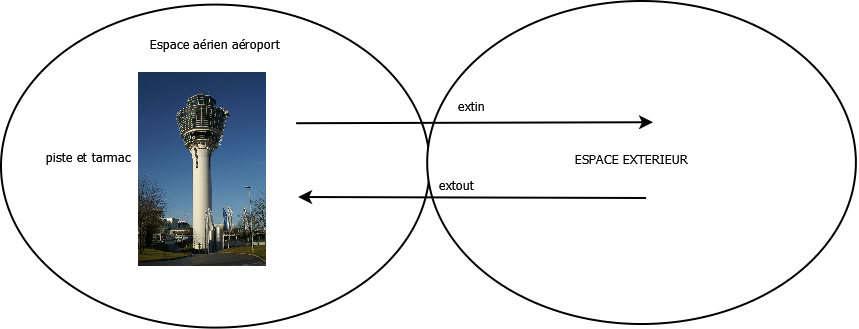
\includegraphics[scale=0.4]{images/mod0}
		\caption{Modèle abstrait}
		\label{mod0}
	\end{center}
\end{figure}

On fait abstraction de la piste. Ainsi, la seule variable à considérer est le nombre d'avions présents sur le tarmac à un instant donné. On note nt cette variable.

\paragraph{Etat static ou \textit{contexte} du système :}
L'état statique est caractérisé par ntmax :
\begin{figure}[H]
	\begin{center}	
		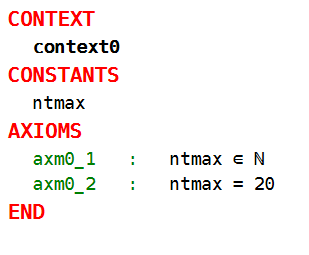
\includegraphics[scale=0.8]{images/ctx0}
		\caption{Etat static du système}
		\label{ctx0}
	\end{center}
\end{figure}

\paragraph{Etat dynamique du système :}
 L'état dynamique du système n'est constitué que de cette seule variable. Elle est définie au moyen de deux conditions ou \textit{invariants} :
%   \begin{align}
%  inv0\_1 : nt \in ℕ 
%   \end{align}
%   
%    \begin{align}
%   inv0\_2 : nt \le ntmax
%   \end{align}
%   

\begin{figure}[H]
	\begin{center}	
		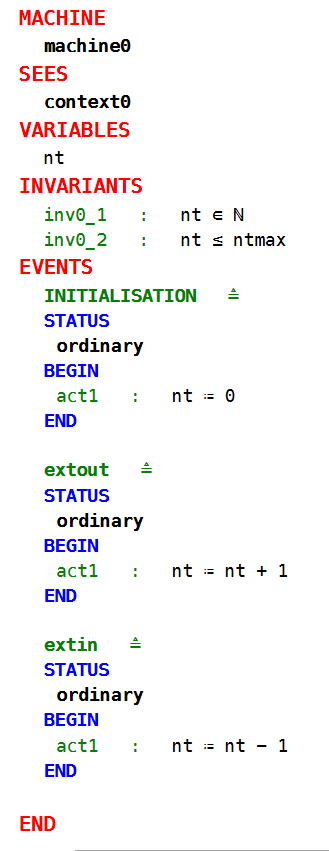
\includegraphics[scale=0.8]{images/mac0}
		\caption{Etat dynamique du système}
		\label{mac0}
	\end{center}
\end{figure}

\begin{figure}[H]
	\begin{center}	
		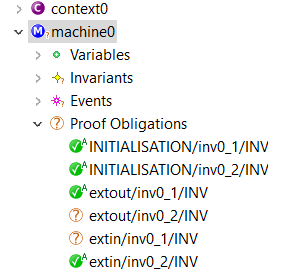
\includegraphics[scale=0.8]{images/proof1}
		\caption{Echec de deux preuves obligatoires}
		\label{proof1}
	\end{center}
\end{figure}

\begin{figure}[H]
	\begin{center}	
		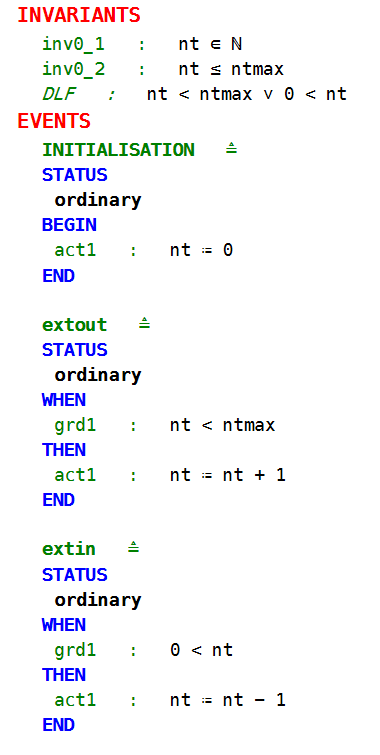
\includegraphics[scale=0.8]{images/garde}
		\caption{Ajout de 2 gardes et d'un théorème pour éviter les blocages}
		\label{garde}
	\end{center}
\end{figure}

\paragraph{conclusion}
Pour débuguer le modèle formel initial, il a fallu ajouter deux gardes pour garantir un nombre d'avions compris entre 0 et 20 et éviter les deadlock. Les exigences sont mises à jour pour tenir compte de ces oublis.

\begin{table} [H]
	
	\centering
	\rowcolors{2}{gray!65}{white}
	\begin{tabu}{|[2pt] p{1.7cm} | [2pt]p{15cm}|[2pt]}
		
		\tabucline[2pt]{-} \rowcolor{yellow}
		\Centering	\textbf{Label}& \Centering \textbf{Exigence}  \\ \tabucline[2pt]{-}
		
		\hline 
		FON-1&Le contrôleur doit autoriser les avions à décoller et atterrir  \\ 
		\hline 
		FON-1.1& \textcolor{red}{Le contrôleur doit fonctionner indéfiniment une fois lancé.}  \\ 
		\hline 
		FON-2	& Le nombre d'avions sur le tarmac est limité à 20 y compris ceux en attente \textcolor{red}{mais doit rester positif} \\ 
		\hline 
		FON-3& Des avions entrent sur et quittent la piste d'atterrissage décollage  \\ 
		\hline 
		FON-4& Des avions entrent sur le tarmac et le quittent  \\ 
		\hline 
		FON-5& La piste ne peut être occupée par plus de un avion \\ 
		\hline 
		FON-6& Le nombre de décollages ou atterrissages successifs n'est pas limité   \\ 
		\hline 
		FON-7& Le contrôleur doit fixer et délivrer les clearances à l'avance   \\ 
		\hline 
		FON-8& Le contrôleur ne doit autoriser l'avion qu'après l'envoi de son identifiant    \\ 
		\hline
		FON-9& Le contrôleur doit soit refuser, soit accepter, soit mettre en attente l'avion demandeur   \\ 
		\hline
		FON-10& Le contrôleur doit refuser la clearance après 10 de mise en attente.   \\ 
		\hline 
		ENV-1 &Tout avion se dirigeant vers la piste doit avoir une autorisation de décoller \\ 
		\hline 
		ENV-2 &Le système est muni d'un capteur qui permet de compter les avions sur la piste \\ 
		\hline 
		ENV-3 &Le système est muni d'un capteur qui permet de compter les avions sur la tarmac \\ 
		\tabucline[2pt]{-}
	\end{tabu} 
	\caption{Tableau des exigences}
\end{table}
